\subsection{Specific Aim 2: Hydrodynamics}
\label{subsec:specific_aim_2}
In Specific Aim 2, we include hydrodynamics effects by embedding the
particles in a solvent.  As described in~\eqref{eq:stokes} and
illustrated in Figure~\ref{fig:flow_map}, the solvent phase is modeled
by the Stokes equations for an incompressible viscous fluid, and these
equations are coupled to the screened-Laplace equation~\eqref{SL}
through viscous and hydrophobic stress balance. Hydrodynamic effects can
not be ignored since the rates of biological functions like fusion,
fission, and pore dynamics rely on viscous
dissipation~\cite{RYHAM20112929}. 
%While hydrophobic attraction causes the particles to self-assemble indepedently of the dissipation mechanism, the trajectories and
%equilibrium configurations depend on the fact that the particles travel through a viscous environment. 
Additionally, hydrodynamic interactions are central for complex
microscopic three-dimensional structures to fabricate~\cite{Cho2010}.
Over the past decade, there has been an explosion of interest in
small-scale processes that utilize capillary forces, van der Waals
interactions, and thermal noise~\cite{Zhang2017}, to coordinate movement
and bind material subunits~\cite{Pandey2011, Leong2007, Reynolds2019,
Dasgupta2017, Siontorou2017}. Finally, coarse-grained and molecular
dynamics theories include water either explicitly or implicitly in their
models. The immediate goal of the present proposal is to simulate
vesicle bilayers in external flows, where the bilayers are represented
by a self-assembled collection of rigid particles.

\begin{figure}[h]
  \centering{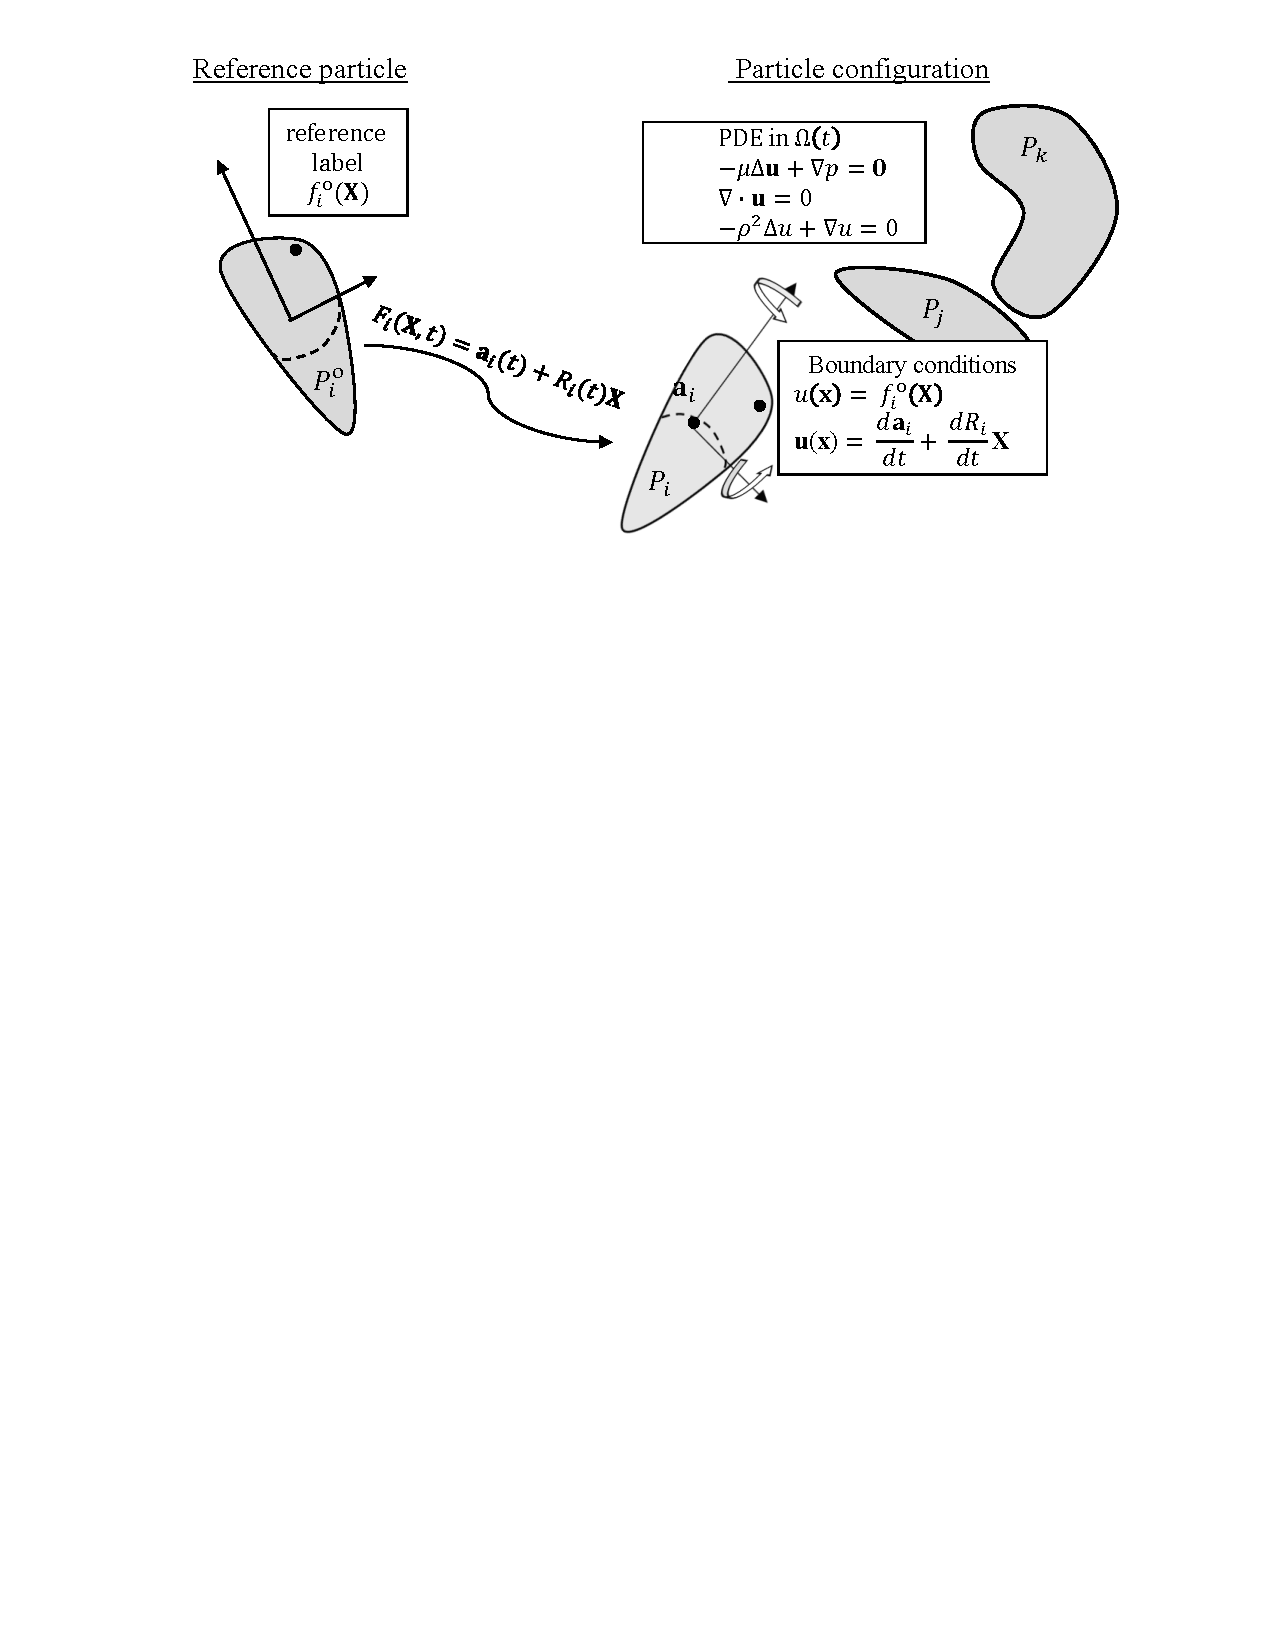
\includegraphics[width=0.8\textwidth]{Figures/domain.pdf}}
    \caption{\label{fig:flow_map}}
\end{figure}


%We must solve the system 
%\setcounter{midequation}{\theequation}
%\addtocounter{midequation}{2}
%\begin{minipage}[t]{0.44\textwidth}
%\begin{subequations}
%\begin{alignat}{2}
%\label{St1} -& \mu \Delta {\bf u} + \nabla p = {\bf 0}, \\
%\label{St2}  & \nabla \cdot {\bf u} = 0,                &&   \text{in } \Omega\\
%\label{St3}  & {\bf u }({\bf x}) = {\bf v}_i + {\bf w_i}\times {\bf x}, \;  && \text{for } {\bf x} \in \partial P_i\\
%\label{St4}  & ({\bf u } - {\bf u}_{\infty})({\bf x}) \to {\bf 0} && \text{as } {\bf x} \to \infty\\
%\notag \\
%\tag{\themidequation}
%\label{HSB1}  & \int_{\partial P_i} \boldsymbol{\sigma} \boldsymbol{\nu} \,\dif S + {\bf F}_{i} = {\bf 0}\span \span
%\end{alignat}
%\end{subequations}
%\end{minipage}
%\addtocounter{equation}{1}
%\setcounter{midequation}{\theequation}
%\addtocounter{midequation}{2}
%\begin{subequations}
%\begin{minipage}[t]{0.5\textwidth}
%\begin{alignat}{2}
%\label{SL1}  - & \rho^2 \Delta u +u = 0, && \text{in } \Omega\\
%\label{SL2}   & u({\bf x}) = f_i({\bf x}),\quad  && \text{for } {\bf x} \in \partial P_i\\
%\label{SL3} &  u({\bf x}) \to 0 && \text{as } {\bf x} \to \infty \\
%\notag \\
%\notag \\
%\tag{\themidequation}
%\label{HSB2}   & \int_{\partial P_i} {\bf x} \times \boldsymbol{\sigma} \boldsymbol{\nu} \,\dif S + {\bf G}_{i} = {\bf 0} \span \span\\
%\notag
%\end{alignat}
%\end{minipage} 
%\end{subequations}
%\noindent for $i = 1,\dots, N$.

\subsubsection{Vesicles in background flows}
Numerically solving the Stokes-screened Laplace system~\eqref{SL}
and~\eqref{eq:stokes} is nontrivial, and we will develop efficient,
robust, high-order in time and space algorithms suited to the problem.
The challenges are: {\bf (1)} the equations express a two-way coupling.
This means that the flow changes the shape of the suspended particles,
and in return the geometry-dependent hydrophobic stresses impart a force
on the flow. {\bf (2)} The inputs to the Stokes equations are particle
configurations, forces, and torques. The outputs are the rigid body
translation and angular velocities used to update the particle positions
(see Figure~\ref{fig:flow_map}). Although the underlying equations are
linear, the overall problem is highly nonlinear because the domain is
constantly changing. {\bf (3)} Self-assembly causes the particles to
come into close contact. As a result, an exceptional spatial accuracy is
required to resolve the fields between adjacent particles. Finally, the
physically relevant elastic properties of bilayer become apparent at
large length scales and for large particle-numbers, which increases the
computational complexity of our simulations. 

We include a background flow by replacing the third equation in
\eqref{eq:stokes} with the condition $(\mathbf{u} -
\mathbf{u}_{\infty})(\mathbf{x}) \to \mathbf{0}$ as $|\mathbf{x}| \to
\infty$. To incorporate the far-field flow, we use the representation 
\begin{align}
\label{PowerMiranda}
  {\bf u} = {\bf u}_{\infty} + K\boldsymbol{\eta} + 
    \sum_{i=1}^N S(\cdot, {\bf a}_i) {\bf F}_i + 
                 R(\cdot, {\bf a}_i) {\bf G}_i.
\end{align}
where $S$ and $R$ are stokeslets and rotlets supported at the respective
particle centers and $K\boldsymbol{eta}$ is a layer potential for the
unknown density function $\boldsymbol{\eta}.$ The
representation~\eqref{PowerMiranda} automatically satisfies all
equations, with the exception of the rigid motion conditions. The rigid
motion conditions follow by requiring the viscous stress vanishes across
the particle boundaries.

We will compare the behavior of our particle-based vesicles in Stokes
flow to well-established results. \todo{What are the known results?}
Researchers have devised models to enforce area incompressibility and
volume conservation in vesicle membrane
dynamics~\cite{torres-sanchez_millan_arroyo_2019,
mahapatra_saintillan_rangamani_2020, Steigmann99, C6SM02452A}. Our
preliminary results show that the particle-based bilayers have the same
large area modulus as real lipid bilayer membranes, so we expect
realistic results from our flow simulations. Under moderate shear rates,
the vesicle elongates and takes on the tank-treading  elliptical shape.
We can directly check for area compressibility conservation properties
from the particle simulation by tracking the change in area density of
the midplane as a function of shear flow rate, along with evaluating the
tangential divergence of the velocity.

Bilayer membranes have a small permeability to water
\cite{323e9a2f0c58487ea82518d7a1f96485}, and modelers often assume a
vesicle membrane that conserves volume. In our particle-based approach,
water motion across the bilayer is limited by the size of the gaps
between the particles, which is an artifact of coarse-graining.  Making
these gaps smaller comes at the expense of numerical accuracy, and we
will assess if there is a reasonable trade-off between approximate
volume conservation and simulation complexity. 

\begin{wrapfigure}[13]{r}{0.30\textwidth}
\centerline{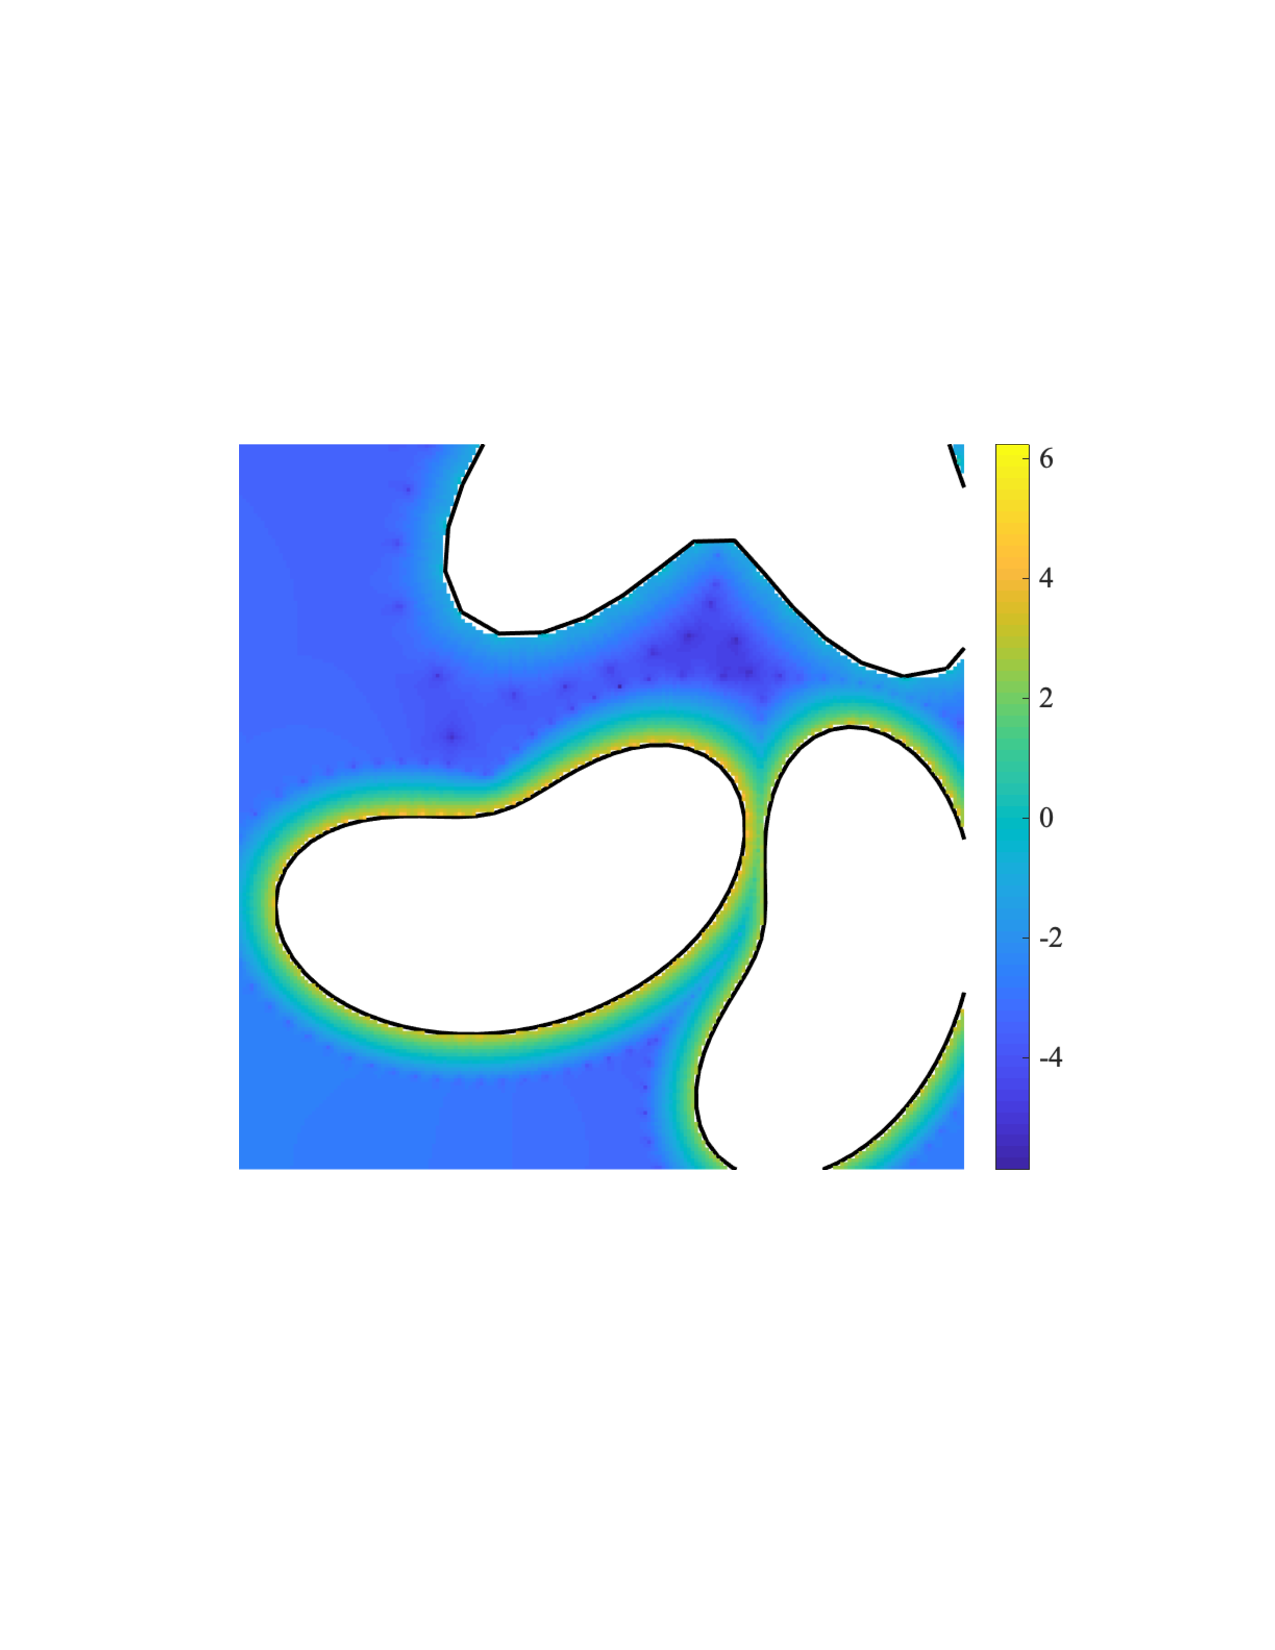
\includegraphics[width=0.30\textwidth]{figures/BIError.pdf}}
  \vspace{-8pt}
\caption{
\label{fig:bierror}  
\footnotesize The false color map shows how numerical quadrature of
  layer potentials loses accuracy near the particle boundaries.  The
  color bar is for $\log_{10}.$}
\end{wrapfigure}

Finally, the particle-based vesicle bilayers have two distinct leaflets
consisting of the particles in contact with the vesicle interior, and
those in contact with the surrounding fluid. Since there is a nonzero
separation between these layers, an important effect we observe is that
the leaflets slide against one another under shear flow.  This implies
that part of the viscous dissipation in the aqueous phase is enhanced by
intermonolayer friction~\cite{SHKULIPA2005823, ShkulipaThesis}.
Intermonolayer slip enters zero-thickness membrane models as a velocity
jump boundary condition and leads to multiple solution
states~\cite{schwalbe_vlahovska_miksis_2010}.  In the present proposal,
intermonolayer slip is an artifact of monolayer independence  and we can
control for slip as a function of shear rate, vesicle diameter, and
particle geometry.

\subsubsection{Novel reciprocal identities}
The force and torque formulas~\eqref{forceandtorque} require the
hydrophobic stress along the particle boundaries. Unfortunately,
standard quadrature formulas to estimate $\nabla u$ on the particle
boundaries introduces large amounts of quadrature error
(Figure~\ref{fig:bierror}). Therefore, it is useful to devise reciprocal
identities for the force and torque on body $i$ that does not
require integration along body $i$. This is achieved using the identity 
\begin{align}
    \label{eq:reciprocal}
{\bf F}_{\text{hydro},i} = \sum_{j \neq i} \int_{\partial P_i}[\boldsymbol{\sigma}_{ij} + \boldsymbol{\sigma}_{ji}]\boldsymbol{\nu}\,\dif S,\quad
{\bf G}_{\text{hydro},i} = \sum_{j \neq i} \int_{\partial P_i} ({\bf
  x}-\mathbf{a}_i) \times [\boldsymbol{\sigma}_{ij} +
  \boldsymbol{\sigma}_{ji}]\boldsymbol{\nu}\,\dif S, 
\end{align}
for $i=1,\ldots,N$, which we have proved. Here $u = \sum_{i=1}^N u_i$ is
a sum of solutions $u_i$ the screened Laplace equation,
$\boldsymbol{\sigma}_{ij} = \rho^{-1} u_iu_j {\bf I} + \rho(\nabla u_i
\cdot \nabla u_j {\bf I} - 2 \nabla u_i \otimes \nabla u_j)$ and
$[\cdot]$ denotes the jump across $\partial \Omega.$  It turns out that
because of \eqref{eq:reciprocal}, we no longer require knowledge of the
gradient on the boundary, which is enormously beneficial for calculating
force and torque.




